\documentclass[paper=letter, fontsize=11pt]{scrartcl} 
 \usepackage[top=2.5cm, bottom=2.5cm, left=2.5cm, right=2.5cm]{geometry}
\usepackage{framed}

\usepackage{graphicx}
\usepackage{verbatim}
\usepackage{pictex}  
\usepackage{multimedia}
\usepackage{listings}
\usepackage{xcolor,colortbl}
\usepackage[spanish]{babel} % language/hyphenation
\usepackage{amsmath,amsfonts,amsthm} % Math packages
\usepackage{amsbsy}
\usepackage{amssymb}
\usepackage{fancyvrb}
\usepackage{sectsty} % Allows customizing section commands
\usepackage[dvipsnames]{xcolor}

\newcommand{\defi}[3]{\textbf{Definición:#3}}
\newcommand{\fin}{$\blacksquare.$}
\newcommand{\finf}{\blacksquare.}

\newcommand{\grstep}[2][\relax]{%
   \ensuremath{\mathrel{
       {\mathop{\longrightarrow}\limits^{#2\mathstrut}_{
                                     \begin{subarray}{l} #1 \end{subarray}}}}}}
\newcommand{\swap}{\leftrightarrow}

\newcommand{\gen}{\text{gen}}

\newtheorem{thmt}{Teorema:}
\newtheorem{thmd}{Definición:}
\newtheorem{thml}{Lema:}
\newtheorem{thmj}{Ejemplo:}
\newtheorem{thma}{Algoritmo:}

\newcommand{\mub}{\mathbf{\mu}}
\newcommand{\xb}{\mathbf{x}}
\newcommand{\Xb}{\mathbf{X}}
\newcommand{\Simgab}{\mathbf{\Sigma}}
\newcommand{\sumk}{\sum_{k=1}^K}
\newcommand{\sumi}{\sum_{i=1}^n}
\newcommand{\sumj}{\sum_{j=1}^n}
\usepackage{biblatex}
\addbibresource{biblio.bib}

\allsectionsfont{\centering \normalfont\scshape} % Make all sections centered, the default font and small caps
\usepackage{float}
\usepackage{fancyhdr} % Custom headers and footers
\pagestyle{fancyplain} % Makes all pages in the document conform to the custom headers and footers
\fancyhead{} % No page header - if you want one, create it in the same way as the footers below
\fancyfoot[L]{} % Empty left footer
\fancyfoot[C]{} % Empty center footer
\fancyfoot[R]{\thepage} % Page numbering for right footer
\renewcommand{\headrulewidth}{0pt} % Remove header underlines
\renewcommand{\footrulewidth}{0pt} % Remove footer underlines
\setlength{\headheight}{13.6pt} % Customize the height of the header
\usepackage{biblatex}
\addbibresource{references.bib}
\numberwithin{equation}{section} % Number equations within sections (i.e. 1.1, 1.2, 2.1, 2.2 instead of 1, 2, 3, 4)
\numberwithin{figure}{section} % Number figures within sections (i.e. 1.1, 1.2, 2.1, 2.2 instead of 1, 2, 3, 4)
\numberwithin{table}{section} % Number tables within sections (i.e. 1.1, 1.2, 2.1, 2.2 instead of 1, 2, 3, 4)

\setlength\parindent{0pt} % Removes all indentation from paragraphs - comment this line for an assignment with lots of text

\newcommand{\horrule}[1]{\rule{\linewidth}{#1}} % Create horizontal rule command with 1 argument of height

\title{	
\normalfont \normalsize 
\textsc{Centro de Investigaci\'on en Matem\'aticas (CIMAT). Unidad Monterrey} 
\\ [25pt] 
\horrule{0.5pt} \\[0.4cm] % Thin top horizontal rule
\huge Tarea 3 \\ 
\horrule{2pt} \\[0.5cm] % Thick bottom horizontal rule
}


\author{Enrique Santibáñez Cortés} % Your name

\date{\normalsize\today} % Today's date or a custom date

\begin{document}
\lstdefinestyle{customc}{
  belowcaptionskip=1\baselineskip,
  basicstyle=\footnotesize, 
  frame=lrtb,
  breaklines=true,
  %frame=L,
  %xleftmargin=\parindent,
  language=C,
  showstringspaces=false,
  basicstyle=\footnotesize\ttfamily,
  keywordstyle=\bfseries\color{green!40!black},
  commentstyle=\itshape\color{red!40!black},
  identifierstyle=\color{blue},
  stringstyle=\color{purple},
}

\lstset{breakatwhitespace=true,
  basicstyle=\footnotesize, 
  commentstyle=\color{green},
  keywordstyle=\color{blue},
  stringstyle=\color{purple},
  language=C++,
  columns=fullflexible,
  keepspaces=true,
  breaklines=true,
  tabsize=3, 
  showstringspaces=false,
  extendedchars=true}

\lstset{ %
  language=R,    
  basicstyle=\footnotesize, 
  numbers=left,             
  numberstyle=\tiny\color{gray}, 
  stepnumber=1,              
  numbersep=5pt,             
  backgroundcolor=\color{white},
  showspaces=false,             
  showstringspaces=false,       
  showtabs=false,               
  frame=single,                 
  rulecolor=\color{black},      
  tabsize=2,                  
  captionpos=b,               
  breaklines=true,            
  breakatwhitespace=false,    
  title=\lstname,             
  keywordstyle=\color{blue},  
  commentstyle=\color{dkgreen},
  stringstyle=\color{mauve},   
  escapeinside={\%*}{*)},      
  morekeywords={*,...}         
} 

\maketitle

\section{Problema 1.}
En este ejercicio es sobre clustering y mezclas de Gaussianas. Considera un modelo de mezclas de $k$ distribuciones
\begin{align*}
    f(x)=\sum_{k=1}^K w_k f_k(x),
\end{align*}
donde $w_k>0$ y $\sum_k w_k=1$. En este caso, supondremos que $f_k=N(\mub_k, \Sigmab_k).$ Supón que tienes datos $\xb_1,\xb_2,\cdots, \xb_n\sim f(x),$ y queremos ajustar el modelo de mezclas de Gaussinas (MMG) para usarlo como un soft$-$clustering.

\subsection{Log$-$verosimilitud de los datos y los estimadores de máxima verosimilitud para los parámetros del modelo.}
Dado que tenemos $\xb_i, \cdots, \xb_n$ in $\mathbf{R}^d$, nuestro objetivo es determinar nuestros parámetos $\theta=\{w_1, \cdots, w_k, \mub_1, \cdots, \mub_k, \Sigma_1, \cdots, \Sigma_k\},$ tenemos que la log$-$verosimilitud de los datos es:
\begin{align*}
    \mathbf{L}(\xb_1,\cdots,\xb_n;\theta)=\log \prod_{i=1}^n P(x_i;\theta)=\sum_{i=1}^n\log \left\[\sum_{k=1}^K p_k f_k(x_i) \right]
\end{align*}
No existe una solución de forma cerrada para encontrar el conjunto de parámetros $\theta$ que maximice esta probabilidad. El algoritmo EM es un algoritmo iterativo que encuentra una solución localmente óptima $\theta$ al problema de maximización de la probabilidad de GMM.\\

\textbf{Paso E}. El Paso E del algoritmo implica encontrar la probabilidad posterior $\gamma_i^k =P(cluster\ k |x_i); \theta)$ de que el punto $x_i$ fue generado por el cluster $k$, para cada $i = 1,\cdots,n$ y $k= 1,\cdots, K$. Este paso asume el conocimiento del conjunto de parámetros $\theta$. Encontramos el posterior usando la regla de Bayes:
\begin{align*}
    \gamma_i^k=\mathbb{P} (C(i)=k|X=x_i)=\frac{w_kf_k(x_i;\theta)}{\sum_k w_k f_l(x_i;\theta}
\end{align*}

\textbf{Paso M.} El paso M del algoritmo maximiza la función de probabilidad logarítmica esperada $\bar{\mathbf{L}}(x_i ,\cdots, x_n;\theta)$, que es un límite inferior en la probabilidad logarítmica. Por tanto, el algoritmo empuja iterativamente hacia arriba la probabilidad de datos.

La función de verosimilitud logarítmica esperada $\bar{\mathbf{L}}(x_i ,\cdots, x_n;\theta)$ es

\begin{align*}
    \bar{\mathbf{L}}(x_i ,\cdots, x_n;\theta)&=\sumi \left[\sumk \gamma_i^k\log \left( \frac{P(x_i,cluster\ k; \theta)}{\gamma_i^k}\right) \right]\\
    &= \sumi \left[\sumk \gamma_i^k\log \left( \frac{w_k f_k(x_i;\theta)}{\gamma_i^k}\right) \right]\\
    &= \sumi \left[\sumk \gamma_i^k\log \left( \frac{w_k \frac{1}{(2\pi)^{d/2}|\Sigma_j|^{1/2}} \exp \left(-\frac{1}{2}(\xb_i-\mub_j)^T\Sigma_j^{-1}(\xb_i-\mub_j) \right)}{\gamma_i^k}\right) \right]
\end{align*}
Ahora calculemos los estimadores de maxima verosimilitud, para ello maximicemos respecto a $\mub_l$:

\begin{align*}
    \frac{\partial\bar{\mathbf{L}}(x_i ,\cdots, x_n;\theta)}{\partial \mub_l}&=\frac{\partial}{\partial \mub_l}\sumi \left[\sumk \gamma_i^k\log \left( \frac{w_k \frac{1}{(2\pi)^{d/2}|\Sigma_j|^{1/2}} \exp \left(-\frac{1}{2}(\xb_i-\mub_j)^T\Sigma_j^{-1}(\xb_i-\mub_j) \right)}{\gamma_i^k}\right) \right]\\
    &= -\frac{\partial}{\partial \mub_l}\sumi \sumk \gamma_i^k\frac{1}{2}(\xb_i-\mub_j)^T\Sigma_j^{-1}(\xb_i-\mub_j)\\
    &= \frac{1}{2}\sumi \gamma_i^k \frac{\partial}{\partial \mub_l} 2\mu_l^T\Sigma_l^{-1}x_i-\mub_ñ^T\Sigma_l^{-1}\mub_l\\
    &=\sumi \gamma_l^j\left( \Sigma_l^{-1}x_i-\Sigma_{l}^{-1}\mubl \right).
\end{align*}
Ahora igualamos a cero y resolvemos para $\mub_l$ tenemos que 
\begin{align*}
    \bf \hat{\mub_l} = \frac{\sumi \gamma_i^k \xb_i}{\sumi \gamma_i^k.}
\end{align*}
Ahora calculemos el estimador de máxima verosimilitud para $w_l$. Agrupando los términos que depende de $w_l$, encontramos que necesitamos maximizar
\begin{align*}
    \sumi \sumk \gamma_i^k\log w_l.
\end{align*}
Sin embargo, sabemos que $\sumi w_i=1$. Entonces tenemos un problema de optimización con restricción, para ello construimos el Lagrangiano
\begin{align*}
    \mathbb{L}(w) = \sumi \sumk \gamma_i^k\log w_j+ \beta \left( \sumj w_j-1\right),
\end{align*}
donde $\beta$ es el mutiliplicador de lagrange. Derivando, tenemos que 
\begin{align*}
    \frac{\partial\mathbb{L}(w)}{\partial w_j} = \sumi \frac{\gamma_i^k}{w_j}+\beta.
\end{align*}
Igualando a cero y resolviento tenemos que,
\begin{align*}
    \hat{w}_j= \frac{\sumi \gamma_i^k}{-\beta}.
\end{align*}
Ahora, usando que sabemos que $\sumi w_i=1$, podemos despejar y obtener que $-\beta = \sumi \sumk w_i^k=\sumi 1 = n.$ Por lo tanto, el estimador de máxima verosimilitud es
\begin{align*}
    \hat{w}_j=\frac{1}{n} \sumi \gamma_i^k.
\end{align*}
De la misma forma que los demás estimadores, tenemos que el estimador de máxima verosimilitud para $\Sigma$ es 
\begin{align*}
    \Sigma_k = \frac{\sumi (x_i-\mu_c)^2\gamma_i^k}{\sumi \gamma_i^k}.
\end{align*}
\subsection{Comparación de resultados}
Para comprobar la eficiencia del modelo de mezclas de Gaussianas usemos un conjunto de datos de sklearn. En este conjunto de datos se observan claramente tres cluster. Si observamos la forma en que están en el espacio, podemos notar que no sería posible utilizar algún método líneal para particionar los tres cluster, por lo que se espera que el algoritmo fuzzy k$-$means tenga una menor eficiencia en este conjunto de datos.\\

Si observamos la Figura \ref{fig:em_gmm}, la cual compara el algoritmo fuzzy k$-$means contra el modelo GMM. Podemos notar claramente la eficiencia que tiene el modelo GMM en comparación del fuzzy k$-$means.

\begin{figure}[H]
    \centering
    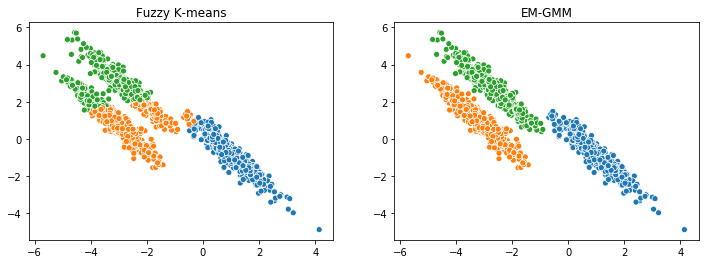
\includegraphics[scale=0.7]{figure/em_gmm.png}
    \caption{Data set: Blob con distintas medias}
    \label{fig:em_gmm}
\end{figure}
En la siguiente sección \ref{compa} realizamos más comparaciones con distintos modelos de clustering y observamos las desventajas que tiene GMM en algunas ocaciones.

\subsection{$\sigma^2\rightarrow 0$}
Para mostrar que cuando $\Simga = \sigma^2\bf I$  y si $\sigma^2\rightarrow 0$ entonces el modelo EM$-$GMM se parece al modelo k$-$means, utilizemos el mismo conjunto de datos solo que cambiemos $\Simga = \sigma^2\bf I$. Es decir, estamos considerando $\Sigma= \begin{pmatrix} 
0.04& 0 & 0\\ 0& 0.0150 & 0 \\ 0 & 0 & 0.09 \end{pmatrix}$ para generar los datos. Observando la figura \ref{fig:em_gmm_var} podemos notar que los clusters construidos por EM$-$GMM son iguales a los de k$-$means. Por lo que si se cumple. Se probaron distintas matriz de varianzas y covarianzas y se sigue cumpliendo para valores pequeños de $\sigma^2.$
\begin{figure}[H]
    \centering
    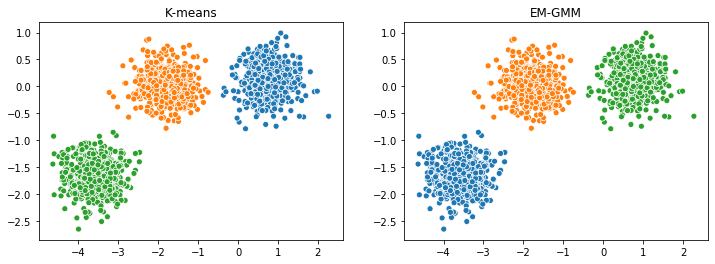
\includegraphics[scale=0.7]{figure/em_gmm_var.png}
    \caption{Data set: Blob con distintas medias y varianza constante}
    \label{fig:em_gmm_var}
\end{figure}

\section{Kernel K$-$means}
Consideremos que tenemos un conjunto de datos $\xb_1, \cdots, \xb_n$ el argoritmo $k-$means trata de encontar $\pi_1, \cdots, \pi_k$ que minicen la función objetivo
\begin{align*}
    \mathbf{D}\left( \left\{ \pi_c\right\}_{c=1}^k\right) = \sum_{c=1}^k \sim_{x_i\in \pi_c} ||x_i-m_c||^2, \text{    donde } m_c=\frac{\sum_{x_i\in\pi_c} x_i}{|\pi_c|}. 
\end{align*}
El kernel $k-$ means usa una función para mapear puntos a un espacio de características de mayor dimensión. Cuando se aplica $k-$means en este espacio de características, los separadores lineales en el espacio de características correponden a separadores no lineales en el espacio de entrada. El objetivo del kernel $k-$means se puede escribir como la minización de
\begin{align*}
    \mathbf{D}\left( \left\{ \pi_c\right\}_{c=1}^k\right) = \sum_{c=1}^k \sim_{x_i\in \pi_c} ||\phi(x_i)-m_c||^2, \text{    donde } m_c=\frac{\sum_{\phi(x_i)\in\pi_c} x_i}{|\pi_c|}. 
\end{align*}
Expendiendo la distancia $||\phi(x_i)-m_c||^2$ en la función anterior obtenemos la siguiente expresión
\begin{align*}
    ||\phi(x_i)-m_c||^2 = \phi(x_i)\cdot \phi(x_i)-\frac{2\sum_{x_i\in \pi_c}\phi(x_i)\cdot \phi(x_j)}{|\pi_c|}+\frac{\sum_{x_j,x_l\in \pi_c} \phi(x_j)\cdot\phi(x_l)}{|\pi_c|^2}
\end{align*}
Entonces, Por lo tanto, solo se utilizan productos internos en el cálculo de la distancia euclidiana entre un punto y un centroide. Como resultado, si se nos da una matriz de núcleo $K$, donde $K_{ij} = \phi(a_i) \cdot \phi(x_j)$, podemos calcular distancias entre puntos y centroides sin conocer representaciones explícitas de $\phi(x_i)$ y $\phi(x_j)$ \cite{kernel_kmeans}.\\

El algoritmo que se utilizo para construir la función kernel $k-$means es el que se describe en \textbf{Algoritmo:} \ref{a_kernel}, solo que con se vectorizar para mejorar la velocidad de ejecución. Es decir, en cada iteración nosotros calculamos todas las distancias del conjunto de datos al cluster $c$. Lo anterior permitió probar con distintos parámetros en las funciones.

\begin{framed}
    \begin{thma} \label{a_kernel}
	\textbf{Entradas:} $X:$ matriz de datos, $K$: matriz kernel, $k$: número de clusters, $t$: número de iteración, $t\_max$: número de iteraciones máximas, ${\pi_c^{(t)}}_{c=1}^k$: vector de la clasificación de los cluster.\\
	\textbf{Ouput:} ${\pi_c^{(t)}}_{c=1}^k$:vector de la clasificación de los cluster en el paso $t+1$.
	\begin{enumerate}
	    \item Para cada punto $x_i$ y para cada cluster $c$, calcular 
	    \begin{align*}
    d(\x_i, m_c) = K_{ii}-\frac{2\sum_{x_i\in \pi_c}K_{ij}}{|\pi_c|}+\frac{\sum_{x_j,x_l\in \pi_c}K_{jl}}{|\pi_c|^2}
\end{align*}

    \item Actualizamos los cluster como
    $$\pi_c^{(t+1)}=\{x:c^*(x_i)=c\}.$$

    \item Si no converge (es decir, comparamos si $\pi_c^{(t+1)}=\pi_c^{(t)}$) o $t\_max>t$ entonces actualizamos $t=t+1$ y regresamos al paso 2. En otro caso, terminamos y retornamos $\{\pi_c^{(t+1)}\}_{c=1}^k.$
	\end{enumerate}
    \end{thma}
\end{framed}

\subsection{Comparación de Resultados} \label{compa}
Utilizamos tres conjuntos de datos diferentes para probar la eficiencia del método kernel $k-$means, estos conjuntos de datos son de la liberaría de python sklearn\cite{scikit-learn}. Para cada conjunto de datos se utilizo kernel k$-$means, k$-$means, fuzzy k$-$means y EM GMM (del inciso anterior), se entrenaron distintos modelos y aquí se muestran los que se consideran como mejores.\\ 

El primer conjunto de datos (Ver figura \ref{fig:all_no_structure}) se pueden observar que estos no tienen ningún patrón, por lo que no existe como una partición de ellos. Observamos que utilizando kernel k$-$means parte los datos en dos segmentos al igual que EM$-$GMM. K$-$means y fuzzy k$-$means parten el conjunto de datos en tres. Para este caso, a todos los modelos se considero el número de cluster igual a 3 ($k=3$).\\

El siguiente conjunto de datos (Ver figura \ref{fig:all_circle}) representa a dos cluster de no lineales (dos círculos diferentes). Se considera como mejor partición de los datos como los dos círculos, por lo que el mejor ajuste se obtiene cuando se usa kernel k$-$means. En este caso se ocupo un kernel polinomial de grado 2, que si recordamos lo visto en clase se obtiene lo mismo.


\begin{figure}[H]
    \centering
    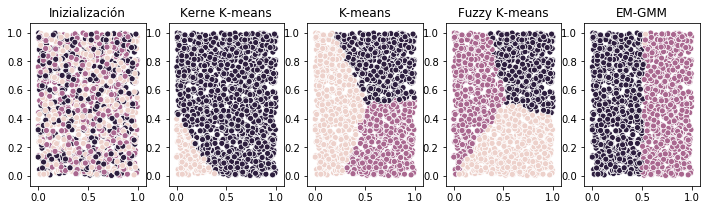
\includegraphics[scale=0.7]{figure/all_no_structure.png}
    \caption{Data set: Sin estructura}
    \label{fig:all_no_structure}
\end{figure}

\begin{figure}[H]
    \centering
    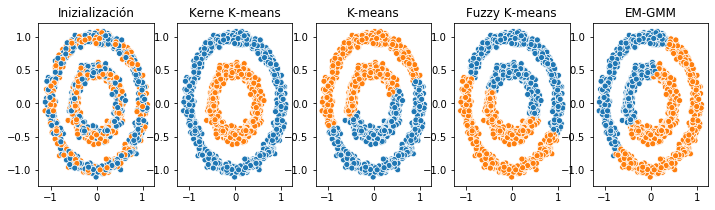
\includegraphics[scale=0.7]{figure/all_circle.png}
    \caption{Data set: circulo.}
    \label{fig:all_circle}
\end{figure}

Ahora consideramos un conjunto de datos en donde claramente se observan tres poblaciones distintas, es decir, visualmente se puede determinar de forma lineal los cluster (Ver figura \ref{fig:all_blob}). En este conjunto de datos, los cuatro algoritmos de clustering logran conseguir los tres cluster. Y por último, el conjunto de medias lunas (Ver figura \ref{fig:all_noisy})
observamos que ningún método de clustering puede clasificar bien este conjunto de datos. Sería recomendable profundizar más con algún otro algoritmo de clasificación (DBSCAN).
\begin{figure}[H]
    \centering
    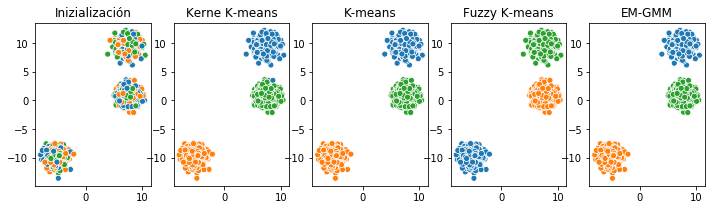
\includegraphics[scale=0.7]{figure/all_blob.png}
    \caption{Data set: Blob}
    \label{fig:all_blob}
\end{figure}

\begin{figure}[H]
    \centering
    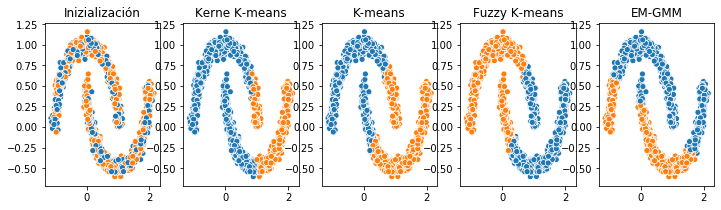
\includegraphics[scale=0.7]{figure/all_noisy.png}
    \caption{Data set: Lunas aleatorias}
    \label{fig:all_noisy}
\end{figure}

\subsection{Conclusiones}
En este ejercicio se mostró la eficiencia del kernel k$-$means, podríamos decir que usar este método en ocasiones cuando existan clusters no lineales aunque esto no es garantía de clasificar bien. Pero si existen una gran ventaja en esta situación que si utilizáramos k$-$means o fuzzy k$-$means, pues recordemos que estos son clasificadores lineales lo que sería imposible para ellos clasificar bien cuando existan patrones no lineas.

\section{Frutas.}
\subsection{Introducción}
Los datos en el archivo \textsc{data}$_$\textsc{fruits}$_$\textsc{tarea.zip} contienen imágenes preprocesadas de $100\times 100$ pixeles, que corresponde a diferentes tipos de frutas, tomadas en diferentes orientaciones y con diferentes características de forma y maduración. En este ejercicio, tratarás de identificar las frutas obteniendo algunas representaciones a partir de las imágenes (Figura 1, por ejemplo).

\subsection{RGM}
Utilizando la representación RGM de las imágenes obtenemos la media de cada color, es decir, teníamos un conjunto de datos de $1300\times 100 \times100$ y lo reducimos a $1300\times 3$.  En la figura \ref{fig:pairplot} podemos observar que las cherry (café) y huckleberry (rosa) se pueden clasificar de manera sencilla utilizando la media del color rojo y azul, estas dos frutas casi no tiene presentes el color rojo por lo que eso explica esa separación entre las demás frutas. Ahora si nos centramos en el color verde (el otro rosa), podemos observar que los aguacates tiene una distribución muy estrecha en comparación de las demás frutas por lo que se podría separar utilizando esta variable.

\begin{figure}[H]
    \centering
    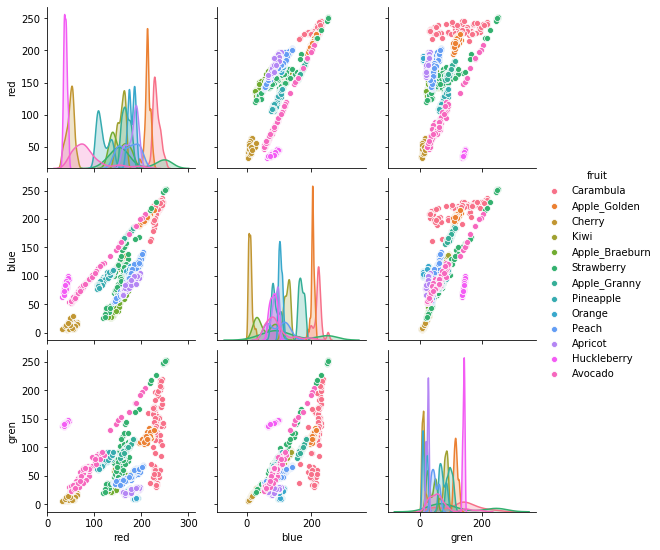
\includegraphics[scale=0.7]{figure/pairplot.png}
    \caption{Gráfica en pares de las medias RGM}
    \label{fig:pairplot}
\end{figure}

\subsection{PCA y Kernel PCA}
Ahora utilizaremos PCA y Kernel PCA (se considero $\alpha=0.2$ en la mayoría de los casos) para reducir la dimensión todavía más, esto para poder vizualizar los datos de una manera sencilla sin perder demasiada información. Graficando los primeros dos componentes principales de ambos métodos, podemos observar nuevamente que los cherries, huckeberry y avocado se pueden clasificar facilmente. En el proyección utilizando PCA podemos ver que la apple golden se puede separar fácilmente. Qué a diferencia de las demás frutas no es tán intuitivo formar los cluster para las 13 frutas.  Observemos que las naranjas y los duraznos están muy cercanos lo que tiene mucho sentido por los colores de las frutas.

\begin{figure}[H]
    \centering
    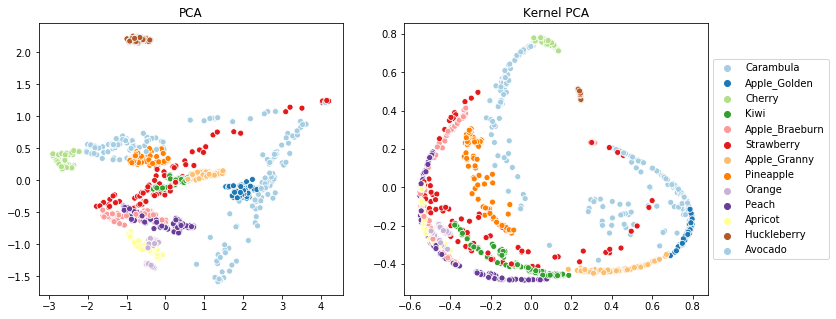
\includegraphics[scale=.6]{figure/pca_rgb.png}
    \caption{PCA y Kernel PCA}
    \label{fig:pca_rgb}
\end{figure}
Consideró que ni PCA como kernel PCA son adecuados para la reducción de la dimensionalidad para este ejercicio, me hubiera gustado probar como TNE o MDS pero por cuestiones de tiempo no pude. 

\subsection{K$-$means y kernel K$-$means} Aplica K$−$means y Kernel K$−$means. Verifica si puedes identificar los diferentes grupos de frutas.

Considerando las proyecciones de la sección anterior, aplicamos k$-$means y kernel k$-$means para intentar clasificar las 13 frutas diferentes. La mejor visualización de k$-$means fue utilizando la proyección PCA, lo cuál tiene sentido ya que realizar una proyección no lineal hace que el algoritmo k$-$means (lineal) no tenga una buena eficiencia. Se comprueba que clasifica bien las frutas mencionadas anteriormente,  (Ver figura \ref{fig:kmeans_pca}) es decir, las cherries, huckleberry las clasifican bien. Los duraznos y naranjas los junta en un mismo cluster.

\begin{figure}[H]
    \centering
    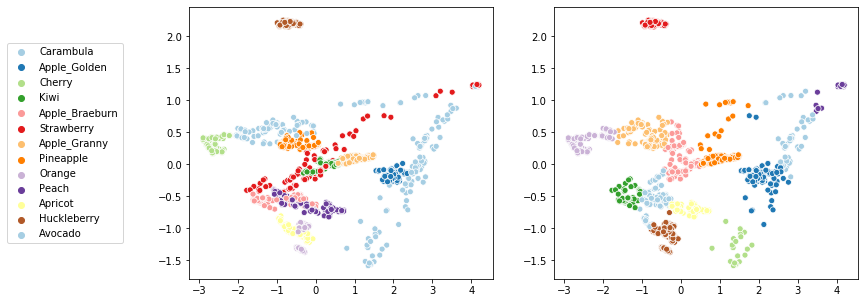
\includegraphics[scale=0.6]{figure/kmeans_pca.png}
    \caption{Kmeans en las proyecciones PCA}
    \label{fig:kmeans_pca}
\end{figure}

Ahora, si consideramos Kernel k$-$means en las proyecciones Kernel PCA algo interesante a observar es que puede clasificar muy bien a las frutas apple brauburn, apricot y apple grammy. Esto se pueda deber a que estas frutas en las proyecciones kernel PCA son no lineales lo que hace posible separarlos utilizando kerner k$-$means.
\begin{figure}[H]
    \centering
    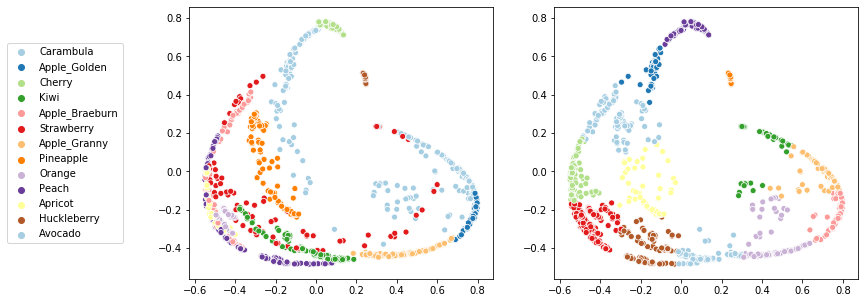
\includegraphics[scale=0.6]{figure/k_means_kpca.png}
    \caption{Kernel k$-$means en las proyecciones Kernel PCA}
    \label{fig:k_kmeans_pca}
\end{figure}

\subsection{Representación usando HSV}
Ahora consideraremos el espacio HSV de las imágenes. En lugar de utilizar solo la mediana como variable, ahora consideraremos los tres cuartiles centrales para cada uno de las dimensiones. Este cambio se espera tener una mayor eficiencia a la hora de clasificar las frutas.\\

Realizamos las proyecciones utilizando PCA y Kernel PCA (Ver figura \ref{fig:pca_hvs}). Para las proyecciones usando PCA podemos observar que huckleberry, pineapple y strawberry son las frutas que posiblemente se puedan separa, que a diferencia de las proyecciones KPCA solo huckleberry y pineable.
\begin{figure}[H]
    \centering
    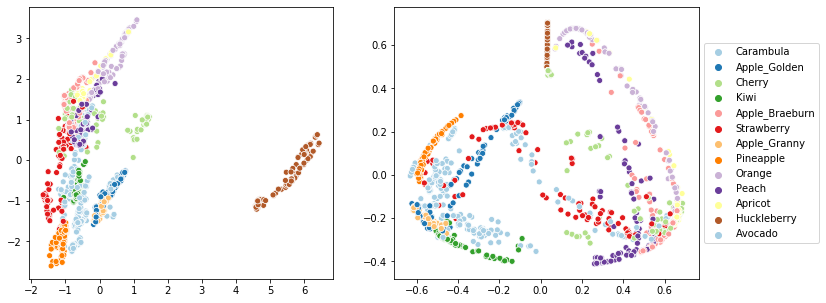
\includegraphics[scale=0.6]{figure/pca_hvs.png}
    \caption{Proyecciones usando PCA y KPCA en HVS}
    \label{fig:pca_hvs}
\end{figure}

Realizando todas las posibles combinaciones de k$-$means, kernel k$-$menas en las proyecciones PCA y KPCA, presentamos mejores resultados. Usando k$-$means usando las proyecciones PCA (Ver Figura \ref{fig:kmeans_pca_hsv}) si comparamos los resultados usando las imágenes en RGB estos no son buenos. Por lo que sería recomendado simplemente utilizar los proyecciones del inciso anterior.
\begin{figure}[H]
    \centering
    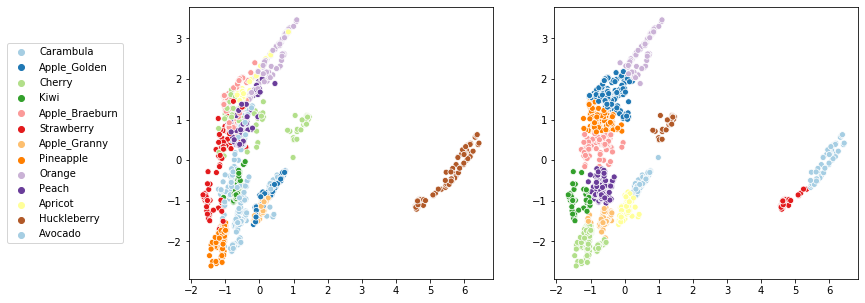
\includegraphics[scale=0.6]{figure/kmeans_pca_hsv.png}
    \caption{K$-$means usando las proyeciones PCA de HVS}
    \label{fig:kmeans_pca_hsv}
\end{figure}
Y ahora, si consideramos Kernel k$-$means usando las proyecciones KPCA podemos clasificar algunas frutas (orange, apple golden) pero la clasificación no sigue siendo muy buena.

\begin{figure}[H]
    \centering
    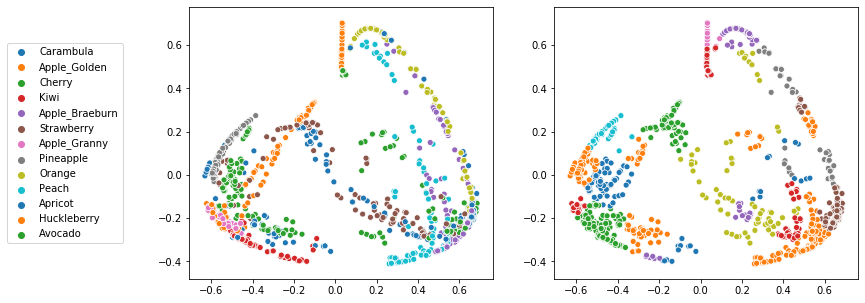
\includegraphics[scale=0.6]{figure/kmeans_kpca_hsv.png}
    \caption{Kernel K$-$means usando las proyeciones KPCA de HVS}
    \label{fig:kmeans_kpca_hsv}
\end{figure}

\subsection{Conclusión}
No se pudo clasificar de manera adecuada todas las frutas, esto puede deberse a la variedad de colores de cada fruta. Como el conjunto de datos tiene tanto frutas maduras como inmaduras, esto hace que sea sencillo confundirse. Por ejemplo, si comparamos el color de una naranja cuando esta madura es muy diferente que cuando no lo esta.\\

Otra razón puede deberse a que los hyperparametros de algoritmos afectan demasiado las clasificaciones. Por hyperparametros me refiero a los valores iniciales del Kernel k$-$means, así como el parámetro que se utiliza al calcular la matriz de distancias. Esto hace que las clasificaciones varíen y no convengan a un mismo mínimo.

\section{Anexos}
\subsection{Códigos}
Todos los códigos utilizados para estos resultados se pueden encontrar en mi página personal de Gitgub: Enriquesec. En el repositorio \texit{ Ciencia$\_$de$\_$Datos/Tareas/Tareas$_$3/}. El archivo EM.py contiene el algoritmo EM para ajustar el modelo de mezclas de Gaussinas. El archivo kernels.py contiene la implementación del kernel k$-$means. Y el notebook homework$_$3.ipnyb contiene las gráficas de este reporte.

\printbibliography

\end{document}